%----------------------------------------------------------------------------
\chapter{Megvalósítás}\label{sect:megvalositas}
%----------------------------------------------------------------------------

A megvalósítás során csak az \textbf{objektumorientált programozás} (object-oriented programming -- OOP) merült fel mint felhasználható módszertan. Az általánosan elterjedt koncepció lehetővé teszi egy komplex probléma kellően intuitív megfogalmazását és átlátható leírását. Erre a fejlesztés során szükség is volt, hiszen a meglehetősen összetetté váló programot csak gondos tervezéssel és kivitelezéssel lehetett megfelelő minőségben előállítani.

Az alkalmazás fejlesztését tehát az OOP paradigmáinak szem előtt tartásával végeztem. Az ismert alapelvek néhány szóban:

\begin{itemize}
  \item \textbf{absztrakció (abstraction):} a probléma valós világbeli objektumok mintájára történő modellezése, a lényegtelen részletek elhagyásával, a lényeges tulajdonságok kiemelésével
  \item \textbf{egységbe zárás (encapsulation):} az egyes osztályok és objektumpéldányok saját maguk rendelkezzenek a futások során szükséges adatok és metódusok felett
  \item \textbf{öröklődés (inheritance):} lehetséges egy általános ősosztály tetszőleges kiegészítése, specializálása a közös elemek megtartásával
  \item \textbf{polimorfizmus (polymorphism):} az egyes műveleteket képesek legyünk bemeneti paraméterek széles skáláján végrehajtani (metódus- vagy operátor-felüldefiniálás)
\end{itemize}

\bigskip

\texttt{+++ melyik szakaszban mi van +++}

%,,,,,,,,,,,,,,,,,,,,,,,,,,,,,,,,,,,,,,,,,,,,,,,,,,,,,,,,,,,,,,,,,,,,,,,,,,,,
\section{Követelmények}\label{sect:kovetelmenyek}
%,,,,,,,,,,,,,,,,,,,,,,,,,,,,,,,,,,,,,,,,,,,,,,,,,,,,,,,,,,,,,,,,,,,,,,,,,,,,

Mielőtt a fejezet későbbi szakaszaiban részletekbe menőben bemutatom az elkészült alkalmazás architektúráját, illetve osztályainak pontos működését, szeretném dokumentálni a kész programra vonatkozó \textbf{követelményeket, azaz specifikációt}.

\bigskip

Az alkalmazás legyen képes:

\begin{enumerate}[a)]
  \item valósidejű \textbf{videofolyamot} olvasni a számítógépre kötött webkameráról (lásd \sectref{infracam} szakasz)
  \item a videofolyam feldolgozásával a \textbf{pupillapozíció meghatározására} a \sectref{pupillakov} szakaszban leírtak szerint.
  \item a tekintet \textbf{kalibrációjára} a \sectref{kalibracio} szakaszban ismertetett módszer felhasználásával.
  \item \textbf{munkamenetek} (session) rögzítésére a képernyő tartalmának mentésével együtt.
  \item a korábbi munkamenetek listázására, törlésére.
  \item munkamenetek \textbf{visszajátszására}.
  \item a munkamenetek alapján \textbf{hőtérképek} generálására (lásd \sectref{web} szakasz)
\end{enumerate}

%,,,,,,,,,,,,,,,,,,,,,,,,,,,,,,,,,,,,,,,,,,,,,,,,,,,,,,,,,,,,,,,,,,,,,,,,,,,,
\section{Architektúra}\label{sect:architektura}
%,,,,,,,,,,,,,,,,,,,,,,,,,,,,,,,,,,,,,,,,,,,,,,,,,,,,,,,,,,,,,,,,,,,,,,,,,,,,
  
  Az implementációt a \sectref{technologia} fejezetben bemutatott technológiák (OpenCV, Qt, Qt Creator) felhasználásával \textbf{C++ nyelven készítettem el} a Model--View--Controller (MVC) tervezési minta szem előtt tartásával. A kialakított osztályhierarchia a \figref{overview} ábrán látható módon épül fel. A kibővített osztálydiagram  -- a fontos változók és funkciók feltüntetésével -- megtalálható az \sectref{osztalydiagram} függelékben.
  
  Az átláthatóság kedvéért még a kibővített diagramról is lehagytam a kevésbé fontos tagváltozókat, és a nyilvánvaló funkcióval rendelkező függvényeket (pl. ,,getter'' vagy ,,setter'' metódusok). Emellett természetesen az információrejtés (information hiding) alapelvének megfelelően a tagváltozók amikor csak szükséges, privát változóként deklaráltak, és publikus interfész áll rendelkezésre az értékük lekérdezésére, vagy az értékadásra.

\begin{figure}[!ht]
\centering
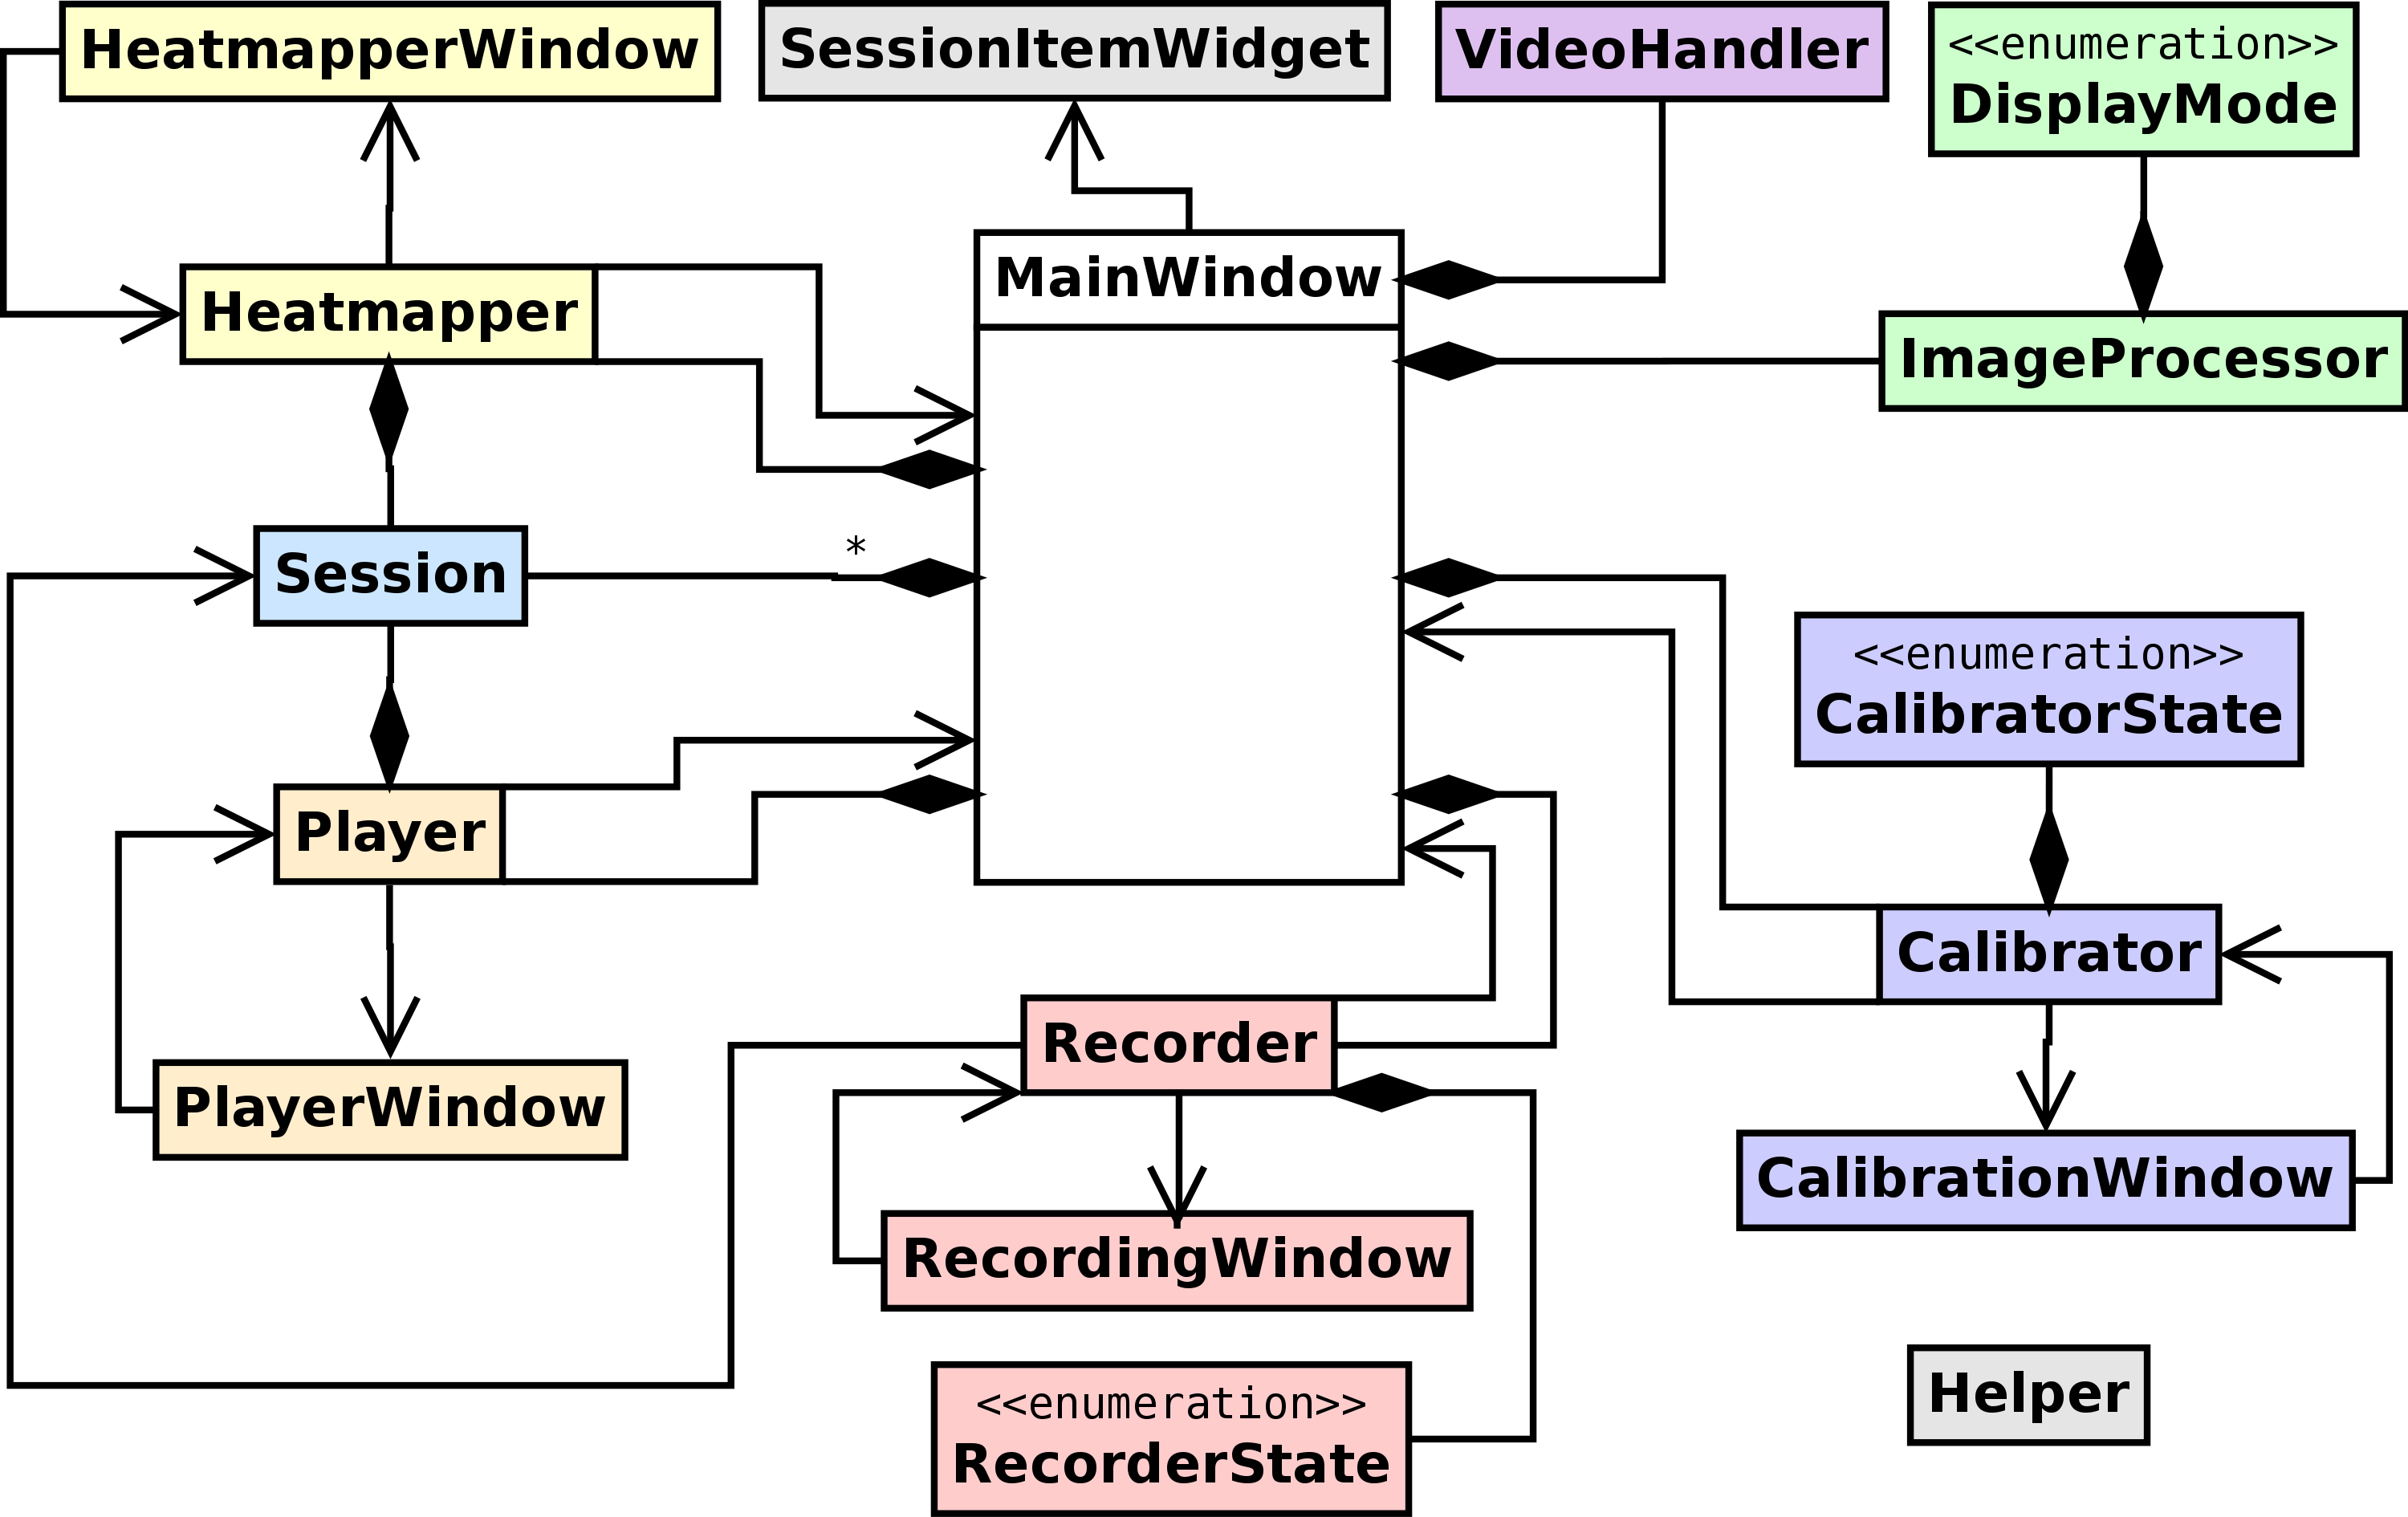
\includegraphics[width=140mm, keepaspectratio]{figures/overview_aa.png}
\caption{Az alkalmazás osztályhierarchiája}
\label{fig:overview}
\end{figure}

Az alkalmazás egyes funkcióit a videofolyam feldolgozásától egészen a hőtérképek generálásáig osztályok egy-egy csoportja végzi. A \figref{overview} ábrán színkódokkal jelöltem a logikailag összetartozó osztályokat. A specifikáció egyes pontjait kielégítő osztályok az ábráról leolvasva, felsorolás szintjén:

\begin{itemize}
  \item \texttt{MainWindow} -- az alkalmazás főablakát tartalmazó osztály, valamint ez szolgál általános kontrollerként is, lévén a felhasználói interakciók döntő része ide fut be
  \item \texttt{VideoHandler} -- a webkameráról beérkező videofolyam olvasásáért felelős
  \item \texttt{ImageProcessor} -- a képkockák feldolgozását -- a pupillakeresést -- végzi
  \item \texttt{Calibrator} -- a kalibrációt, majd kalibrált állapotban a \emph{pupilla-pozíció} $\Longrightarrow$ \emph{képernyő-pozíció} átszámítást végzi
  \item \texttt{Recorder} -- a munkamenetek rögzítését végzi
  \item \texttt{Player} -- a felvett munkamenetek visszajátszását teszi lehetővé ez az osztály
  \item \texttt{Heatmapper} -- a hőtérképek generálása történik ebben az osztályban
  \item \texttt{Session} -- konténerosztály egy-egy munkamenet futásidejű tárolása számára
  \item kisegítő osztályok
\end{itemize}

A továbbiakban sorra veszem az egyes osztályok interfészét, valamint belső működésüket, kicsit mélyebb betekintést engedve a felépítésükbe, egymással való összeköttetésükbe, valamint az esetleg érdekesnek ítélhető implementációs részletekbe.

%............................................................................
\subsection{A \texttt{MainWindow} osztály}\label{sect:mainwindow}
%............................................................................

\begin{figure}[!ht]
\centering
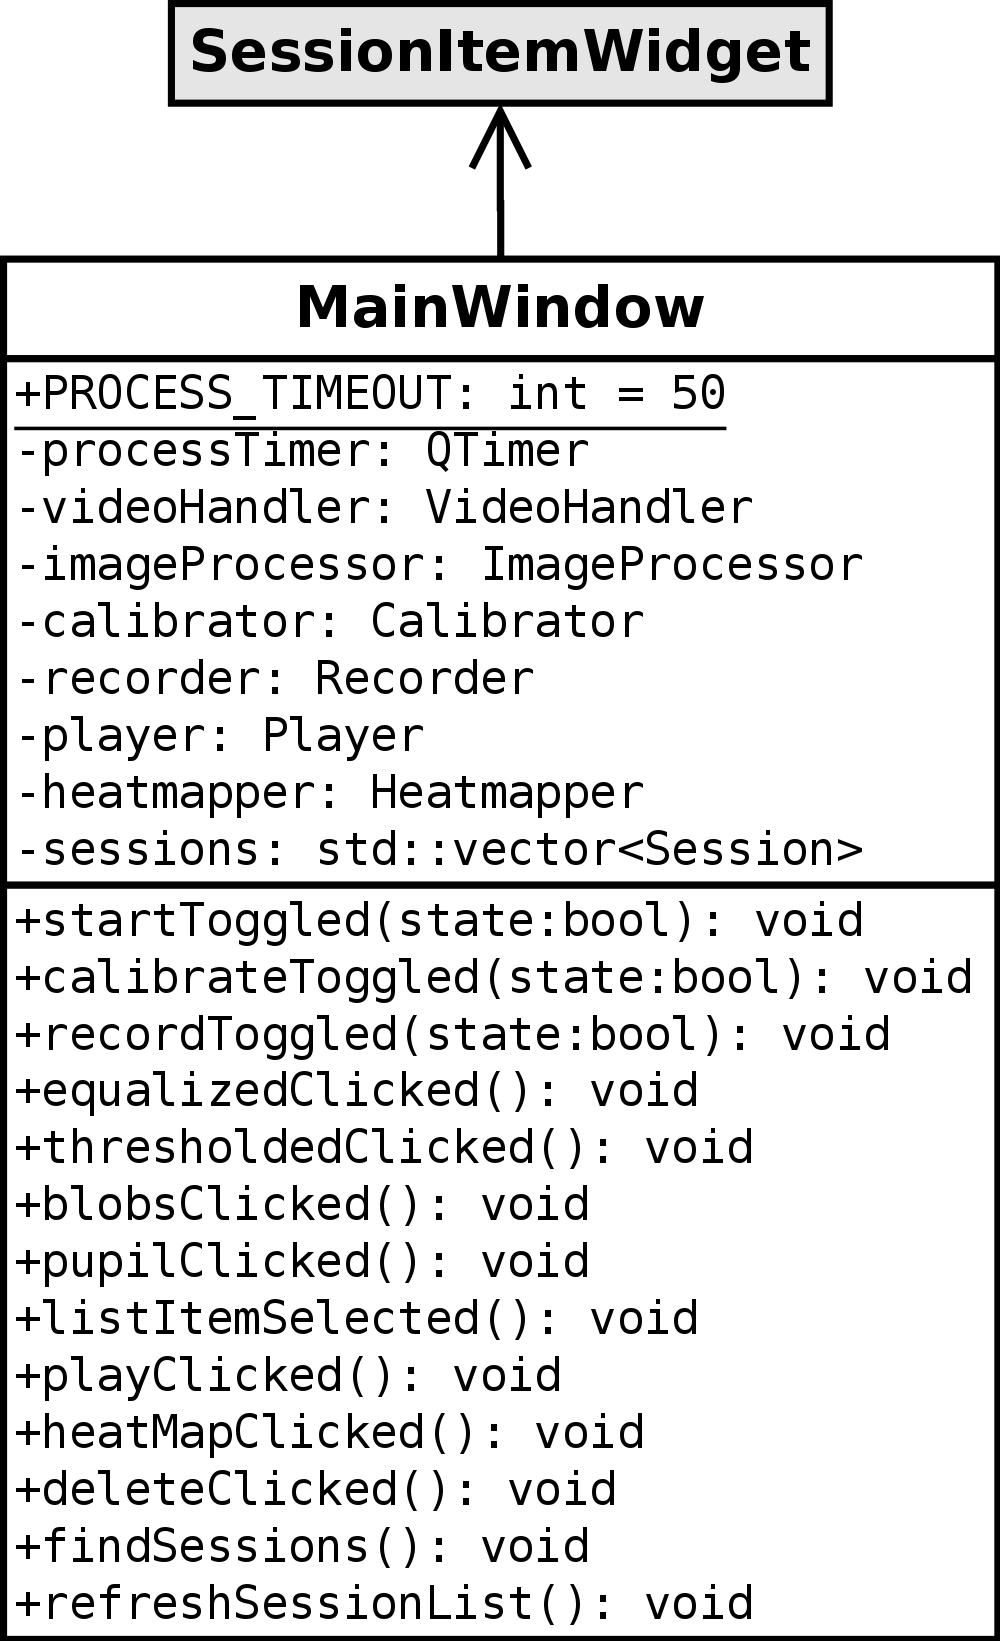
\includegraphics[width=50mm, keepaspectratio]{figures/class_mainwindow.png}
\end{figure}

A \texttt{MainWindow} osztály az alkalmazás általános kontrollereként működik. A nevéből is látszik, hogy ehhez az osztályhoz tartozik a program fő interfészablaka, ennek megfelelően a felhasználói interakciók lekezelése ezen osztály slotjaiban történik. Az osztályban tényleges feldolgozás nem történik, csak összefogja az egyes lépéseket elvégezni hivatott objektumokat, valamit biztosítja, hogy a felhasználói felület állapota mindig a program tényleges belső állapotát reprezentálja, és csak engedélyezett állapotátmenetek történhessenek.

\bigskip

Az \texttt{int PROCESS\_TIMEOUT} attribútum a \texttt{QTimer processTimer} időzítővel együtt a feldolgozás rögzített sebességgel történő elvégzését vezérli. Az előbbi ezredmásodpercben megadott értéke alapján hívódik a feldolgozást vezérlő \texttt{processTimeout} függvény.

A \texttt{sessions} lista az elmentett munkamenetek futásidejű tárolására szolgál, amely listát a \texttt{refreshSessionList} függvény állítja elő.

A \texttt{videoHandler}, \texttt{imageProcessor}, \texttt{calibrator}, \texttt{recorder}, \texttt{player} és \texttt{heatmapper} attribútumok tárolják a névből adódó típusú objektumpéldányokat, amelyek az alkalmazás egyes funkcióit valósítják meg.

A metódusok közül a \texttt{startToggled}, \texttt{calibrateToggled} és \texttt{recordToggled} metódusok sorra a videofolyam, kalibráció és a felvétel ki/bekapcsolását kezelik le.

A lejátszás során megjelenítési módok váltását kezelik le az \texttt{equalizedClicked} és a \texttt{pupilClicked} között felsorolt függvények.

%............................................................................
\subsection{A \texttt{VideoHandler} osztály}\label{sect:videohandler}
%............................................................................

\begin{figure}[!ht]
\centering
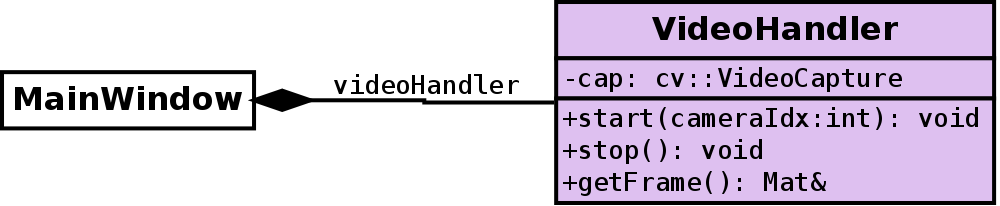
\includegraphics[width=80mm, keepaspectratio]{figures/class_videohandler.png}
\end{figure}

A \texttt{VideoHandler} az ,,alacsony szintű'' videokezelést végzi. A gyakorlatban ez úgy valósul meg, hogy \texttt{cv::VideoCapture cap} attribútumaként tartalmazza az OpenCV kamerakép-feldolgozásra szolgáló objektumának egy példányát.

A \texttt{start} függvényét egy kameraindexszel paraméterezve inicializálhatjuk a fent említett objektumot, a \texttt{stop} függvény pedig a kamera szabályos leállítására szolgál.

Elindított állapotban a \texttt{getFrame} függvénnyel kérhetjük le az adott pillanatban a kamera által érzékelt képet. A képet tartalmazó \texttt{cv::Mat} objektumpéldány szintén az osztály egy tagváltozójában kerül tárolásra, a \texttt{getFrame} függvény erre az objektumra mutató referenciát ad vissza. A megoldásnak nyilvánvalóan performanciabeli okai vannak: a tényleges objektumpéldány átadása felesleges számításokat róna a feldolgozási sorra.

%............................................................................
\subsection{Az \texttt{ImageProcessor} osztály}\label{sect:imageprocessor}
%............................................................................

\begin{figure}[!ht]
\centering
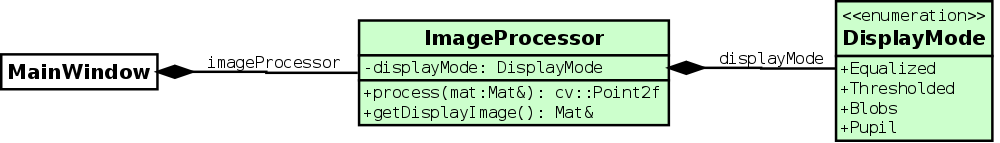
\includegraphics[width=140mm, keepaspectratio]{figures/class_imageprocessor.png}
\end{figure}

Az \texttt{ImageProcessor} osztály végzi a képkockák feldolgozását, és a pupilla azonosítását. A pupillakeresést az alkalmazás előfeldolgozás után blobok detektálásával és változatos szűrésével végzi, a \sectref{pupillakov} szakaszban részletesen bemutatott módon.

A \texttt{process} függvény végzi a felismerés, és a képen megtalált pupillaközépponttal tér vissza egy \texttt{cv::Point2f} változó használatával. A visszaadott középpont az érvénytelen $(-1, -1)$ koordinátákat kapja, ha nem sikerült a pupilla azonosítása.

Szükség van még ezen kívül a feldolgozás valamely közbülső állapotának képét lekérésére, ezt tehetjük meg a \texttt{getDisplayImage} metódus használatával. A függvény az \texttt{ImageProcessor} belső \texttt{displayMode} állapotának megfelelően adja vissza a kívánt képet. Fontos megjegyezni, hogy mindez csak a megjelenítést befolyásolja. A \texttt{displayMode} állapottól függetlenül a pupillafelismerés folyamata minden esetben elejétől a végéig lefut, majd visszatér a megtalált pupillaközéppont koordinátáival.
 
%............................................................................
\subsection{A \texttt{Calibrator} osztály}\label{sect:calibrator}
%............................................................................

\begin{figure}[!ht]
\centering
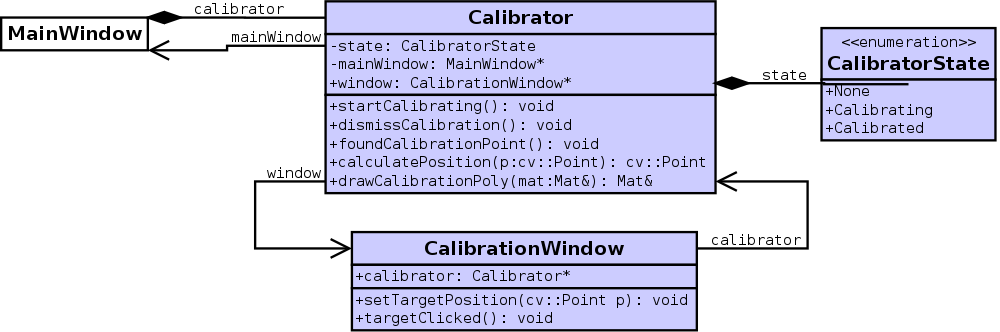
\includegraphics[width=140mm, keepaspectratio]{figures/class_calibrator.png}
\end{figure}

A \texttt{Calibrator} osztály az alkalmazás kalibrálását, majd a pupilla-koordináta alapján a képernyőn éppen nézett pont koordinátájának kiszámítását végzi. A kalibráció folyamatát részletesen a \sectref{kalibracio} szakaszban ismertettem.

Az osztályhoz tartozik egy \texttt{CalibrationWindow} objektum is, amely a futás során dinamikusan kerül lefoglalásra (ezért csak a rámutato pointert tároljuk). Emellett a kalibrálás állapotát is nyilvántartjuk, erre szolgálnak a \texttt{CalibratorState} felsorolás (enumeration) értékei: nincs kalibrálva (\texttt{None}), kalibrálás alatt (\texttt{Calibrating}), vagy kalibrálva (\texttt{Calibrated}).

\bigskip

A \texttt{startCalibrating} és \texttt{dismissCalibration} függvények elnevezései magukért beszélnek. A \texttt{dismissCalibration} függvény elveti a meglévő kalibrációs paramétereket, a \texttt{startCalibrating} metódus esetében pedig új kalibrációt indítunk: megnyílik a \texttt{CalibratorWindow} osztály felhasználói felülete (teljes képernyős kalibrációs ablak), rajta az első kalibrációs ponttal.

A kalibrációs ablakban tekintetünket az aktuális pontra irányítva, majd kattintva (\texttt{targetClicked}) a \texttt{foundCalibrationPoint} függvény hívása történik meg, amelyben utasításra kerül a következő kalibrációs pont kirajzolása \texttt{setTargetPosition}, vagy az utolsó pont esetén a kalibráció lezárása.

\bigskip

Kalibrált állapotban a \texttt{calculatePosition} függvény a \texttt{cv::Point} formában paraméterül adott pupillakoordinátát képzi le a kalibrációs paraméterek felhasználásával képernyő-koordinátákba.

\bigskip

Az \texttt{ImageProcessor} osztályhoz hasonlóan itt is az interfész részét képezik olyan metódusok, amelyek nem feltétlenül a tekintetkövetés szempontjából elengedhetetlen számítási feladatokat végeznek, csak a megjelenítés miatt van szükség rájuk. A \texttt{Calibrator} osztály esetében ilyen a \texttt{drawCalibrationPoly} függvény, amely a paraméteréül kapott képre egyszerűen rárajzolja a kalibrációs pontok négyszögét.

%............................................................................
\subsection{A \texttt{Session} osztály}\label{sect:session}
%............................................................................

\begin{figure}[!ht]
\centering
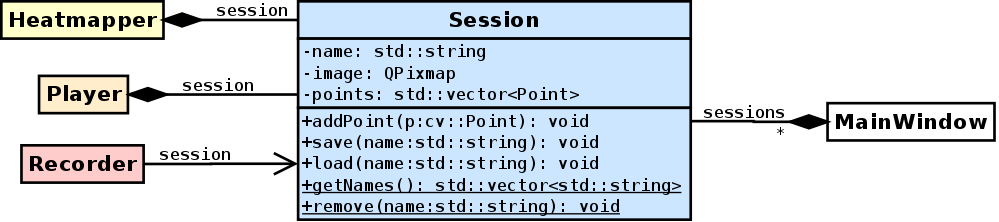
\includegraphics[width=140mm, keepaspectratio]{figures/class_session.png}
\end{figure}

A \texttt{Session} osztály az éppen felvétel alatt lévő, és már felvett munkamenetek futás közbeni tárolására szolgál.

Tagváltozóként tartalmazza a munkameneteket jellemző tulajdonságokat: a munkamenet nevét (azonosítóját, tetszőleges \texttt{std::string name}, a képet, amelyet a felvétel alatt az alany vizsgál (\texttt{QPixmap} objektumként), valamint a vizsgálat alatt felvett képernyő-koordinátákat (\texttt{std::vector<cv::Point> points} listaként).

\bigskip

A publikus interfészen keresztül lehetőség van a munkamenet-objektum lementésére a \texttt{save} metódus használatával. A paraméterül adott azonosítóval kerül lementésre a munkamenet, a futtatási könyvtár \texttt{session\_<név>} formátumú alkönyvtárába. A munkamenet alkönyvtárán belül létrejön a \texttt{bg.png} képfájl, ami értelemszerűen a vizsgálat alatt használt képet tartalmazza, valamint a \texttt{points.txt} szöveges fájl, amely  soronként tartalmazza a rögzített pontok képernyő-koordinátáit.

A mentés párjaként a \texttt{load} függvény tölti be a paraméterül kapott névvel lementett munkamenetet.

\bigskip

A fentieken kívül két statikus metódus is helyet kapott a \texttt{Session} osztályban. A \texttt{getNames} függvény a már lementett munkamenetek neveinek tömbjét adja vissza, a \texttt{remove} osztálymetódus pedig visszavonhatatlanul törli a háttértárról paraméterként megadott névvel rendelkező munkamenetet.

%............................................................................
\subsection{A \texttt{Recorder} osztály}\label{sect:recorder}
%............................................................................

\begin{figure}[!ht]
\centering
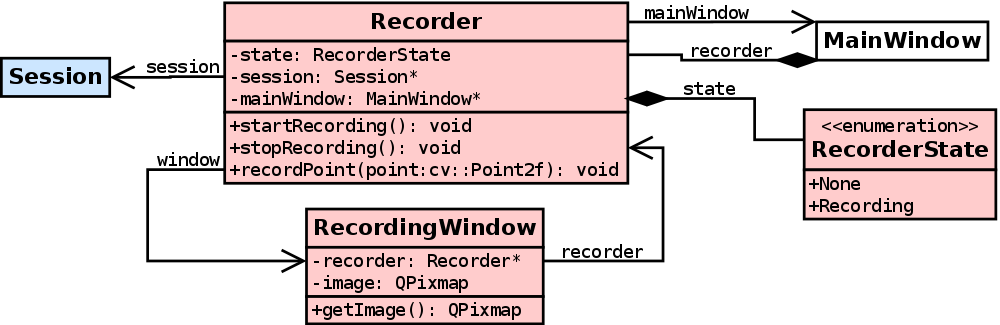
\includegraphics[width=140mm, keepaspectratio]{figures/class_recorder.png}
\end{figure}

A \texttt{Recorder} osztály felelős az új munkamenetek létrehozásáért. Tartozik hozzá egy, a megjelenítést végző ablak, a \texttt{RecordingWindow} osztály egy példánya. Emellett a belső állapot is nyilvántartásra kerül a \texttt{RecorderState} felsorolás értékei által.

Az osztály publikus interfésze mondhatni magától értetődő. A \texttt{startRecording} függvény a meghívását követően azonnal képernyőképet (screenshot) készít az elsődleges kijelző tartalmáról, és elkezdi egy új munkamenet felvételét. A munkamenet azonosítója az alkalmazás jelenlegi állapotában automatikusan a felvétel indításának pillanatában érvényes UNIX időbélyeg (timestamp) értéke lesz.

A \texttt{recordPoint} metódussal új mérési pontot lehet a munkamenethez fűzni. Az alkalmazás használata során a \texttt{recordPoint} függvény felvétel során minden képkocka feldolgozása után meghívódik, vagyis képkockánként egy mérési pont kerül tárolásra. Ennél sűrűbb mintavételnek nyilvánvalóan nincs értelme, de a ritkább pontregisztrálás lehetősége adott.

A \texttt{stopRecording} függvény a felvétel befejeztével hívódik meg. A futása során eltünteti a felvételi ablakot, valamint le is menti az elkészült munkamenetet a háttértárra.

%............................................................................
\subsection{A \texttt{Player} osztály}\label{sect:player}
%............................................................................

\begin{figure}[!ht]
\centering
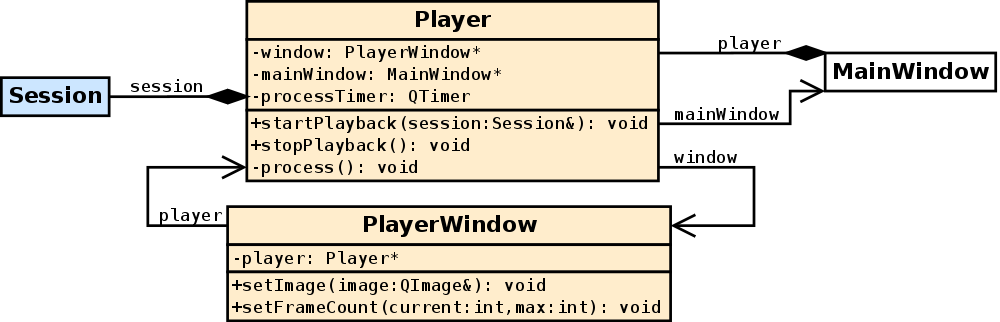
\includegraphics[width=140mm, keepaspectratio]{figures/class_player.png}
\end{figure}

A \texttt{Player} osztály a felvett munkamenetek lejátszásáért felelős. A lejátszást a dinamikusan foglalt \texttt{PlayerWindow} példány grafikus felületén végzi.

A \texttt{startPlayback} metódus egy munkamenet-objektumra (\texttt{Session}) mutató referenciát vár paraméterként, ennek lejátszását kezdi el meghívása után azonnal.

A visszajátszás futása közben a \texttt{processTimer} időzítő és a \texttt{process} függvény gondoskodik a megfelelő ütemben történő visszajátszásról, felhasználva a \texttt{MainWindow} osztály \texttt{PROCESS\_TIMEOUT} értékét. A feldolgozott képet a \texttt{PlayerWindow} osztály \texttt{setImage} metódusának meghívásával jeleníti meg.

A \texttt{stopPlayback} függvény egyszerűen bezárja a használt (teljes képernyős) ablakot, ezzel egy időben leállítja a munkamenet visszajátszását.

%............................................................................
\subsection{A \texttt{Heatmapper} osztály}\label{sect:heatmapper}
%............................................................................

\begin{figure}[!ht]
\centering
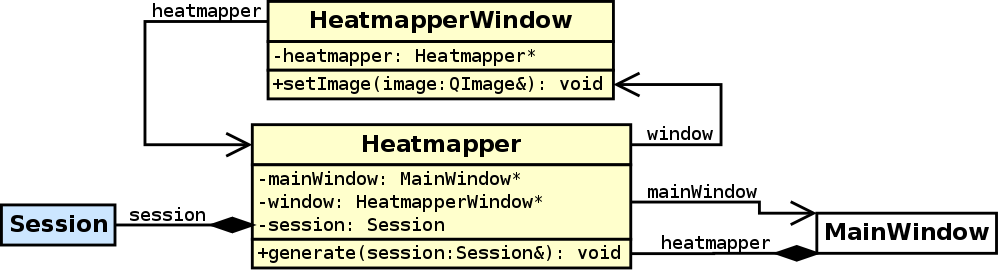
\includegraphics[width=140mm, keepaspectratio]{figures/class_heatmapper.png}
\end{figure}

A \texttt{Heatmapper} osztály a munkamenetekhez kapcsolódó hőtérképek (heatmap) generálására és megjelenítésére szolgál.

Az osztály \texttt{generate} függvénye a paraméterül kapott \texttt{Sesssion} referencia alapján kezdi meg a működését. A generálás meglehetősen hosszú folyamat, ennek végeztével a \texttt{HeatmapperWindow} osztály grafikus felületén jelenik meg a munkamenet hőtérképes reprezentációja.

%............................................................................
\subsection{Kisegítő osztályok}\label{sect:helper}
%............................................................................

Röviden szeretnék szót ejteni az osztálydiagram eddig mellőzött elemeiről is. Ezek az osztályok nem közvetlenül a specifikáció valamely pontjára nyújtanak megoldást, inkább ismétlődő feladatok megoldására adnak helyet.

\paragraph{A \texttt{SessionItemWidget} osztály}

Az osztály a megjelenítésben jut szerephez. A munkamenetek egy listában kerülnek megjelenítésre a főablak bal oldalán. A lista elemeinek egyedi megjelenítésük van, ennek a grafikus elemnek (widget) a felületét tartalmazza a \texttt{SessionItemWidget} osztály.

\paragraph{A \texttt{Helper} osztály}

A kódolás során több helyen is szükség volt különböző átalakítások elvégzésére. A \texttt{Helper} osztály statikus metódusai időbélyegek formázására, valamint a Qt és az OpenCV belső kép-reprezentációi közötti oda-vissza átalakításra szolgálnak.

%,,,,,,,,,,,,,,,,,,,,,,,,,,,,,,,,,,,,,,,,,,,,,,,,,,,,,,,,,,,,,,,,,,,,,,,,,,,,
\section{Grafikus felhasználói felület}\label{sect:gui}
%,,,,,,,,,,,,,,,,,,,,,,,,,,,,,,,,,,,,,,,,,,,,,,,,,,,,,,,,,,,,,,,,,,,,,,,,,,,,

\texttt{+++ leiras + kepek a felhasznalo feluletrol +++}

%,,,,,,,,,,,,,,,,,,,,,,,,,,,,,,,,,,,,,,,,,,,,,,,,,,,,,,,,,,,,,,,,,,,,,,,,,,,,
\section{Felhasználói dokumentáció}\label{sect:docs}
%,,,,,,,,,,,,,,,,,,,,,,,,,,,,,,,,,,,,,,,,,,,,,,,,,,,,,,,,,,,,,,,,,,,,,,,,,,,,

Az alkalmazás indítása után a felhasználót a főablak fogadja. Az ablak bal oldalán a felvett munkamenetek megtekintésére, törlésére, lejátszására, illetve hőtérkép generálására van lehetőség. A főablak jobb oldalán van lehetőség új munkamenetek rögzítésére.

\paragraph{Munkamenet felvétele}

\begin{enumerate}
  \item Adjuk fel a vizsgálandó alanyra a sapkát, amelyhez a webkamera rögzítve van!
  \item Végezzük el a kamerakép bekapcsolását a \textbf{Start} gomb megnyomásával (gyorsbillenyű: \textbf{S})!
  \item Győződjünk meg róla, hogy a kamera orientációja megfelelő: ha nem, irányítsuk a szemrégióra!
  \item Szükség esetén állítsuk be a kamera fókuszát a lencse tekerésével úgy, hogy a pupilla a lehető legélesebben rajzolódjon ki!
  \item Kérjük meg az alanyt, hogy a vizsgálat során csak a szemét mozgassa, a fejét ne! A pontosabb mérés érdekében használhatunk álltámaszt is.
  \item Indítsuk a kalibrációt a \textbf{Calibrate} gomb megnyomásával (gyorsbillentyű: \textbf{C})!
  \item A kalibráció során kérjük meg az alanyt, hogy tekintetét irányítsa a képernyő sarkain sorban megjelenő céltáblákra! A kalibrációs pont rögzítését a céltáblára kattintva, vagy az \textbf{Enter} gyorsbillentyű segítségével végezhetjük.
  \item A háttérben jelenítsük meg a vizsgálni kívánt képet (pl. weboldal részlete).
  \item A \textbf{Record} gomb megnyomásával indítsuk el a munkamenet felvételét (gyorsbillentyű: \textbf{R})
  \item A felvételt a \textbf{Record} gomb újbóli megnyomásával, vagy az \texttt{Escape} gyorsbillentyűvel állíthatjuk le.
\end{enumerate}

\paragraph{Munkamenet visszajátszása}

\begin{enumerate}
  \item Válasszuk ki a bal oldali listából a visszajátszani kívánt munkamenetet!
  \item Kattintsunk a \texttt{Play} gombra! A visszajátszás megkezdődik, és folyamatosan ismétlődik, amíg le nem állítjuk.
  \item A visszajátszás leállításához nyomjuk meg az \textbf{Escape} billentyűt!
\end{enumerate}

\paragraph{Hőtérkép generálása}

\begin{enumerate}
  \item Válasszuk ki a bal oldali listából azt a munkamenetet, amelyhez hőtérképet szeretnénk generálni!
  \item Kattintsunk a \textbf{Heatmap} gombra! A generálás megkezdődik, a folyamat állása a státuszsávon visszajelzésre kerül. A generálás végeztével a hőtérkép megjelenik a képernyőn.
  \item Használjuk az \textbf{Escape} billentyűt a hőtérkép bezárásához.
\end{enumerate}

\paragraph{Többmonitoros használat}

A program fel lett készítve a több monitorral történő használatra. Amennyiben nem a saját tekintetünket követjük, hanem egy másik felhasználóét (alany), úgy a kétmonitoros elrendezés használata a legkényelmesebb.

Az alkalmazás főablakát húzzuk a másodlagos monitorra, ez lesz a vizsgáló képernyője. Az elsődleges monitort használjuk az alany képernyőjeként, azon jelenítsük meg a vizsgálni kívánt ábrákat, képeket, weboldal-részleteket stb. A másodlagos monitoron a vizsgáló a mérés teljes időtartama alatt szemmel tarthatja az alkalmazás főablakát. Ennek köszönhetően például azt is figyelemmel kísérheti, hogy a kamera vagy a fej elmozdulásából kifolyólag a kalibráció a mérés során (vagy két mérés között) helytelenné válik-e. Amennyiben igen, kérheti új kalibráció elvégzését és a mérés megismétlését.

%,,,,,,,,,,,,,,,,,,,,,,,,,,,,,,,,,,,,,,,,,,,,,,,,,,,,,,,,,,,,,,,,,,,,,,,,,,,,
\section{Tesztelés, eredmények}\label{sect:teszteles}
%,,,,,,,,,,,,,,,,,,,,,,,,,,,,,,,,,,,,,,,,,,,,,,,,,,,,,,,,,,,,,,,,,,,,,,,,,,,,

\texttt{+++ tesztelesi dokumentacio (ide mit?) +++}